% 2007 年江西卷理科第 7 题：棱长为 1 的正方体 AC1，AH⊥平面 A1BD，H 为垂足。
%   图中标出 A、B、C、D、A1、B1、C1、D1、H 与平面 A1BD。
% 来源 PDF：gaokaomath-src/普通高考/2007/2007江西理.pdf
% SHA-256：6602cbc393b02e9940beb0035be6e2a28d88a77e0e7792260dcd4c873b542a82
% 原页：2007江西理.pdf 第 1 页（A3 三栏）第 3 栏，书页码 385。
% 重绘依据：按原页正方体斜投影、平面 A1BD 与垂足 H 的位置重绘。
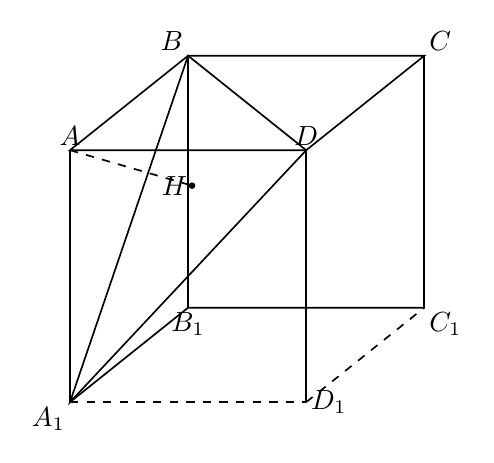
\begin{tikzpicture}[scale=1.0, semithick,
  every node/.style={inner sep=1.5pt}]

  \coordinate (A)  at (0,3.2);
  \coordinate (B)  at (1.5,4.4);
  \coordinate (C)  at (4.5,4.4);
  \coordinate (D)  at (3.0,3.2);
  \coordinate (A1) at (0,0);
  \coordinate (B1) at (1.5,1.2);
  \coordinate (C1) at (4.5,1.2);
  \coordinate (D1) at (3.0,0);

  % 被遮挡的棱
  \draw[dashed] (A1) -- (D1);
  \draw[dashed] (D1) -- (C1);
  \draw[dashed] (D1) -- (D);

  % 可见的棱
  \draw (A) -- (B) -- (C) -- (D) -- cycle;
  \draw (A) -- (A1);
  \draw (B) -- (B1);
  \draw (C) -- (C1);
  \draw (D) -- (D1);
  \draw (A1) -- (B1) -- (C1);

  % 平面 A1BD 与垂足 H
  \draw (A1) -- (B) -- (D) -- cycle;
  \coordinate (H) at (1.55,2.75);
  \draw[dashed] (A) -- (H);
  \fill (H) circle (1.2pt);

  \node[above] at (A) {$A$};
  \node[above left] at (B) {$B$};
  \node[above right] at (C) {$C$};
  \node[above] at (D) {$D$};
  \node[below left] at (A1) {$A_1$};
  \node[below] at (B1) {$B_1$};
  \node[below right] at (C1) {$C_1$};
  \node[right] at (D1) {$D_1$};
  \node[left] at (H) {$H$};
\end{tikzpicture}
